\begin{appendices}
	
\chapter{PIT maven code}
\label{ap:PIT_maven_code}
Example of code used to execute a full set of mutants with PIT.
\begin{lstlisting}
    <plugins>
      <plugin>
        <groupId>org.pitest</groupId>
        <artifactId>pitest-maven</artifactId>
        <version>1.6.4</version>
        <dependencies>
          <dependency>
            <groupId>com.niverhawk</groupId>
            <artifactId>pitest-clustering-plugin</artifactId>
            <version>1.0-SNAPSHOT</version>
          </dependency>
        </dependencies>
        <configuration>
          <exportLineCoverage>true</exportLineCoverage>
          <mutators>
            <mutator>ALL</mutator>
          </mutators>
          <threads>6</threads>
        </configuration>
      </plugin>
\end{lstlisting}

\chapter{Box-plots of samples per project with all characteristics n*0.25 reduction}
\label{ap:full_25}
\begin{figure}[h]
    \centering
    \subfloat{{\includegraphics[scale=0.32]{images/full_25/boxplot_google-auto-service.png}}}
    \qquad
    \subfloat{{\includegraphics[scale=0.32]{images/full_25/boxplot_scribejava-core.png}}}
\end{figure}

\begin{figure}[h]
    \centering
    \subfloat{{\includegraphics[scale=0.3]{images/full_25/boxplot_google-auto-factory.png}}}
    \qquad
    \subfloat{{\includegraphics[scale=0.3]{images/full_25/boxplot_google-auto-common.png}}}
\end{figure}

\begin{figure}[h]
    \centering
    \subfloat{{\includegraphics[scale=0.3]{images/full_25/boxplot_google-auto-value.png}}}
    \qquad
    \subfloat{{\includegraphics[scale=0.3]{images/full_25/boxplot_gson.png}}}
\end{figure}

\begin{figure}[h]
    \centering
    \subfloat{{\includegraphics[scale=0.3]{images/full_25/boxplot_commons-io.png}}}
    \qquad
    \subfloat{{\includegraphics[scale=0.3]{images/full_25/boxplot_commons-cli.png}}}
\end{figure}

\begin{figure}[h]
    \centering
    \subfloat{{\includegraphics[scale=0.3]{images/full_25/boxplot_commons-text.png}}}
    \qquad
    \subfloat{{\includegraphics[scale=0.3]{images/full_25/boxplot_commonc-codec.png}}}
\end{figure}

\begin{figure}[h]
\centering
\includegraphics[scale=0.3]{images/full_25/boxplot_commons-csv.png}
\end{figure}

\chapter{Box-plots of samples per project with all characteristics n*0.50 reduction}
\label{ap:full_50}
\begin{figure}[h]
    \centering
    \subfloat{{\includegraphics[scale=0.32]{images/full_50/boxplot_google-auto-service.png}}}
    \qquad
    \subfloat{{\includegraphics[scale=0.32]{images/full_50/boxplot_scribejava-core.png}}}
\end{figure}

\begin{figure}[h]
    \centering
    \subfloat{{\includegraphics[scale=0.3]{images/full_50/boxplot_google-auto-factory.png}}}
    \qquad
    \subfloat{{\includegraphics[scale=0.3]{images/full_50/boxplot_google-auto-common.png}}}
\end{figure}

\begin{figure}[h]
    \centering
    \subfloat{{\includegraphics[scale=0.3]{images/full_50/boxplot_google-auto-value.png}}}
    \qquad
    \subfloat{{\includegraphics[scale=0.3]{images/full_50/boxplot_gson.png}}}
\end{figure}

\begin{figure}[h]
    \centering
    \subfloat{{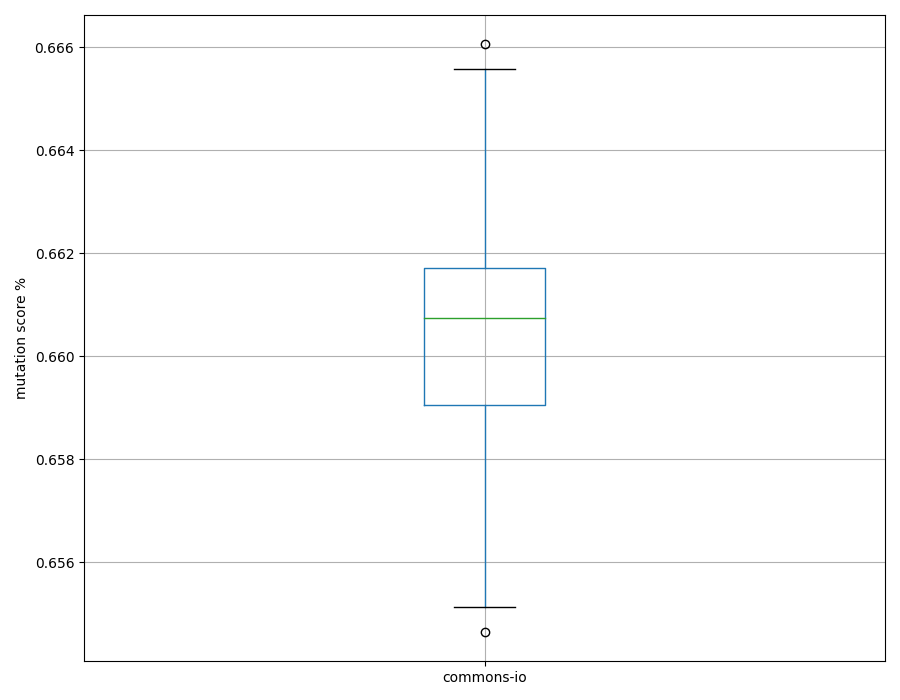
\includegraphics[scale=0.3]{images/full_50/boxplot_commons-io.png}}}
    \qquad
    \subfloat{{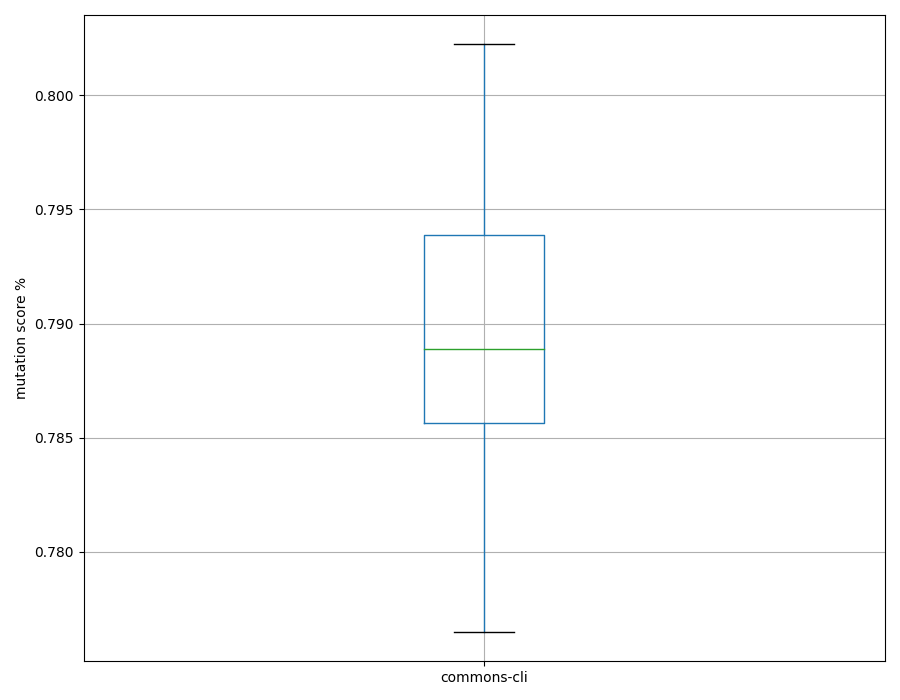
\includegraphics[scale=0.3]{images/full_50/boxplot_commons-cli.png}}}
\end{figure}

\begin{figure}[h]
    \centering
    \subfloat{{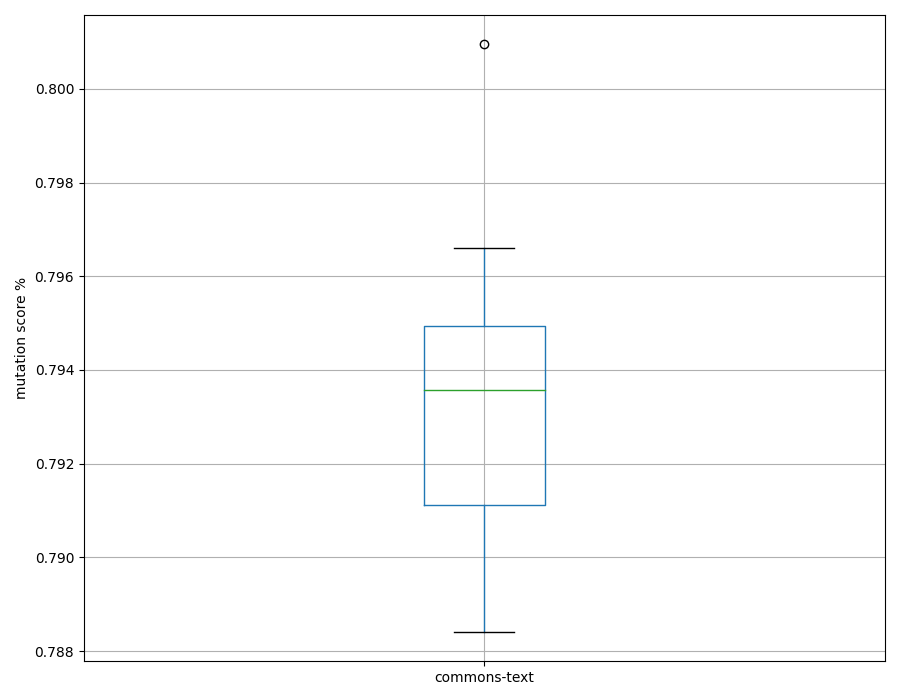
\includegraphics[scale=0.3]{images/full_50/boxplot_commons-text.png}}}
    \qquad
    \subfloat{{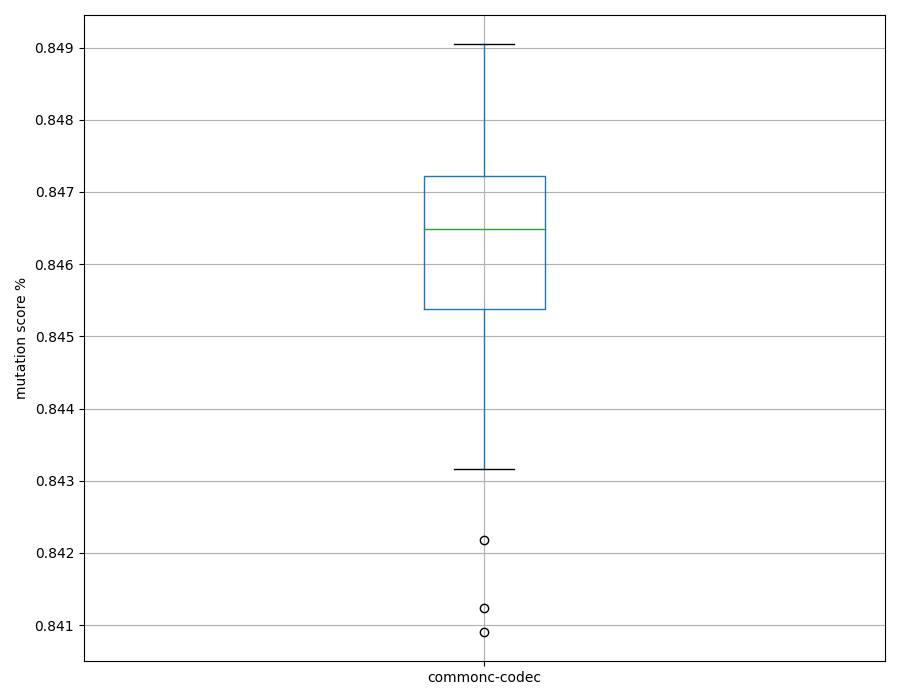
\includegraphics[scale=0.3]{images/full_50/boxplot_commonc-codec.png}}}
\end{figure}

\begin{figure}[h]
\centering
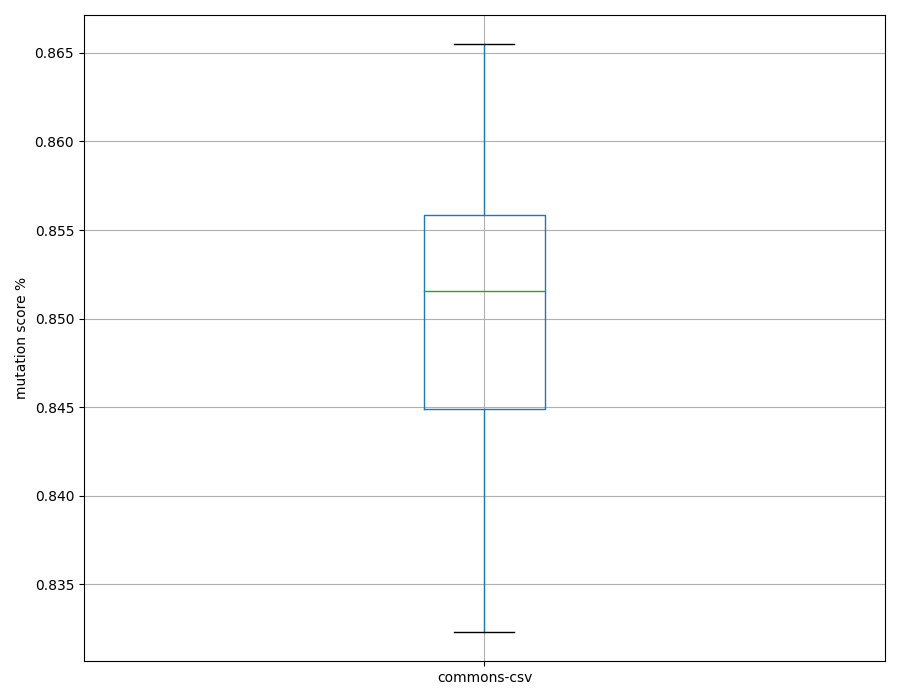
\includegraphics[scale=0.3]{images/full_50/boxplot_commons-csv.png}
\end{figure}

\chapter{Box-plots of samples per project with all characteristics n*0.75 reduction}
\label{ap:full_75}
\begin{figure}[h]
    \centering
    \subfloat{{\includegraphics[scale=0.32]{images/full_75/boxplot_google-auto-service.png}}}
    \qquad
    \subfloat{{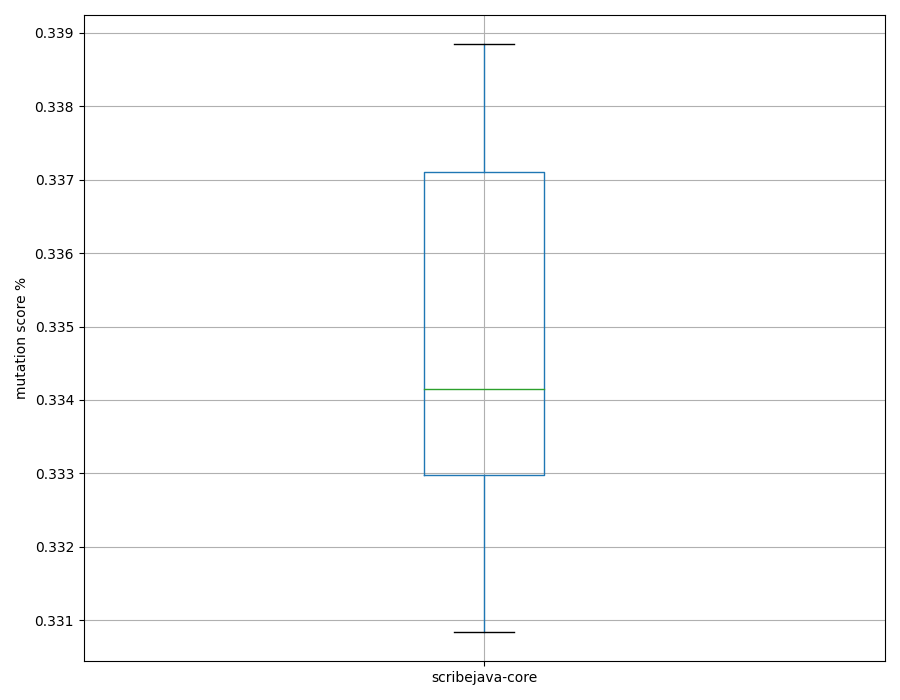
\includegraphics[scale=0.32]{images/full_75/boxplot_scribejava-core.png}}}
\end{figure}

\begin{figure}[h]
    \centering
    \subfloat{{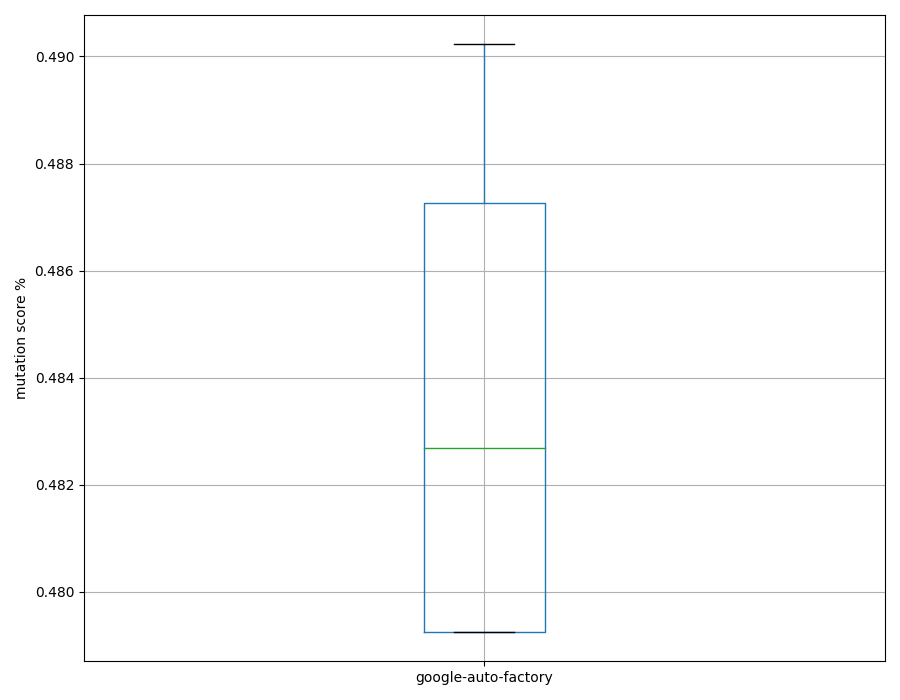
\includegraphics[scale=0.3]{images/full_75/boxplot_google-auto-factory.png}}}
    \qquad
    \subfloat{{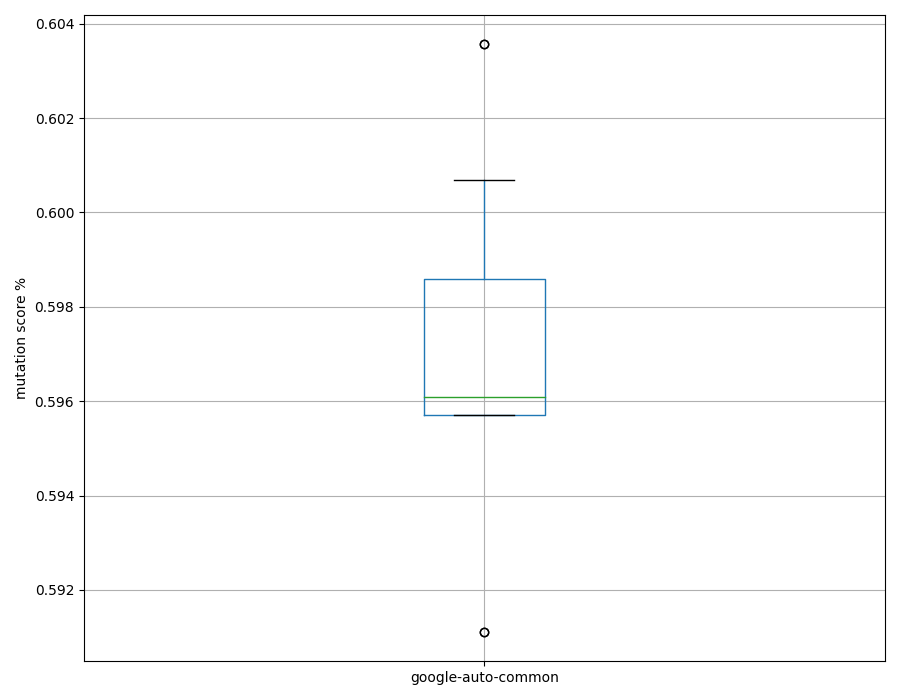
\includegraphics[scale=0.3]{images/full_75/boxplot_google-auto-common.png}}}
\end{figure}

\begin{figure}[h]
    \centering
    \subfloat{{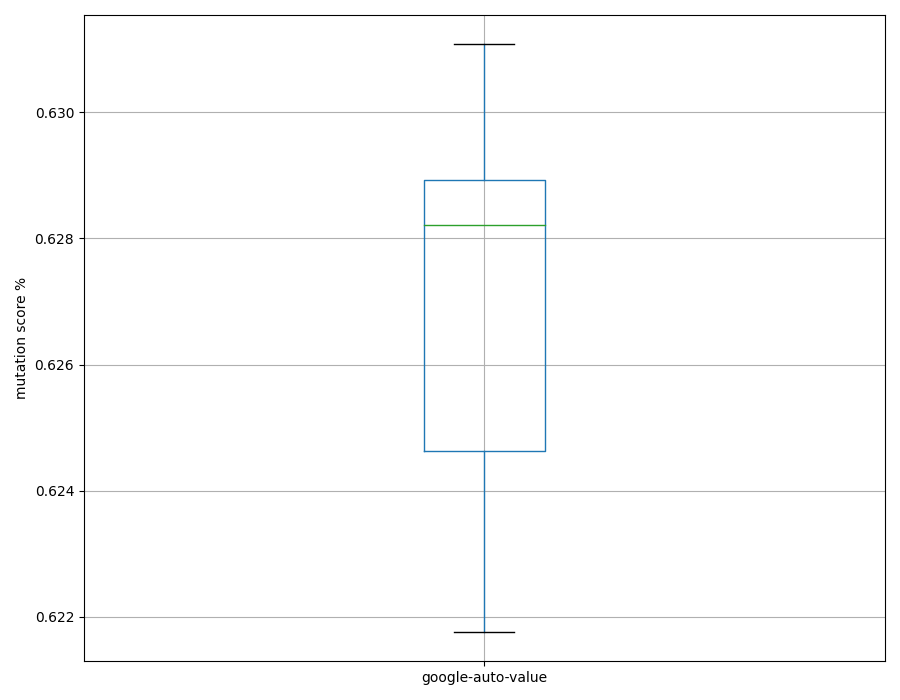
\includegraphics[scale=0.3]{images/full_75/boxplot_google-auto-value.png}}}
    \qquad
    \subfloat{{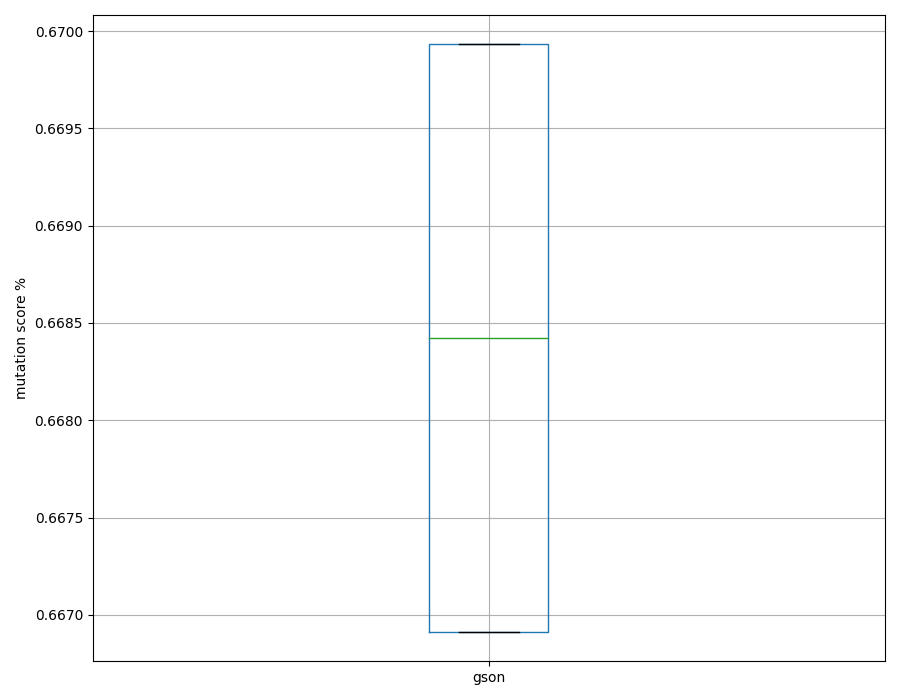
\includegraphics[scale=0.3]{images/full_75/boxplot_gson.png}}}
\end{figure}

\begin{figure}[h]
    \centering
    \subfloat{{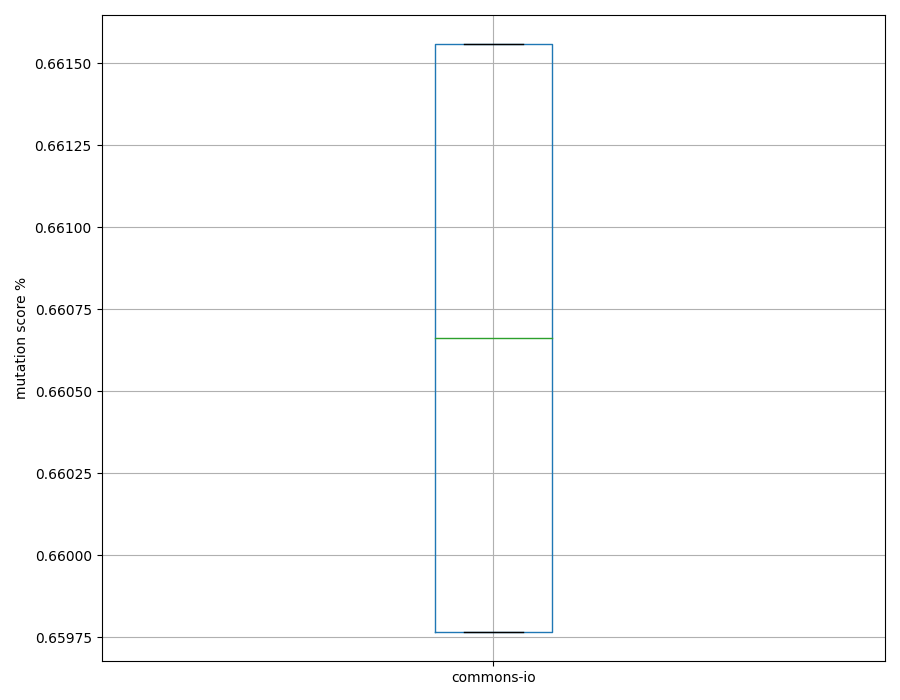
\includegraphics[scale=0.3]{images/full_75/boxplot_commons-io.png}}}
    \qquad
    \subfloat{{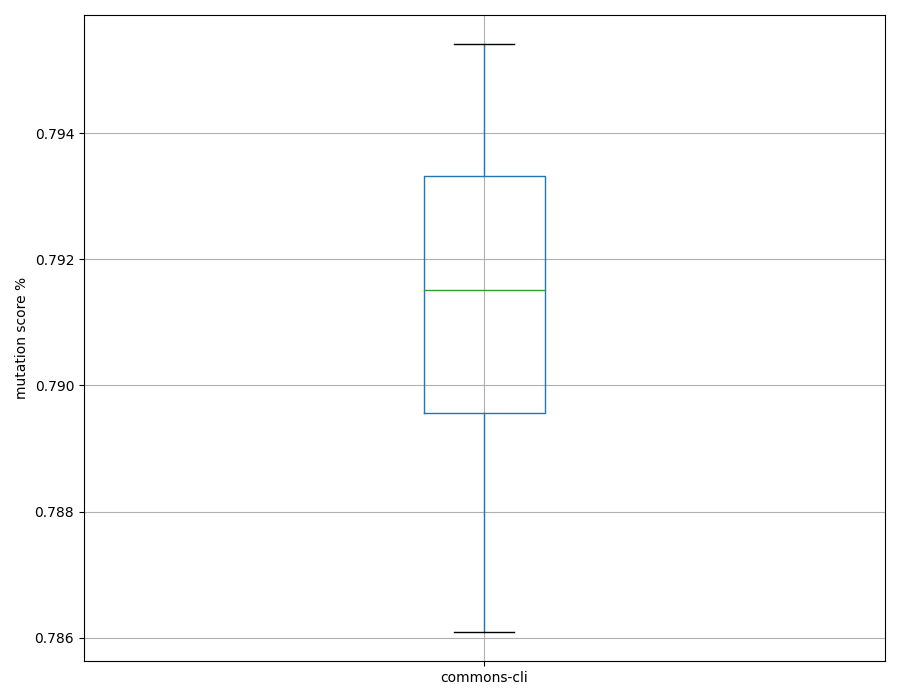
\includegraphics[scale=0.3]{images/full_75/boxplot_commons-cli.png}}}
\end{figure}

\begin{figure}[h]
    \centering
    \subfloat{{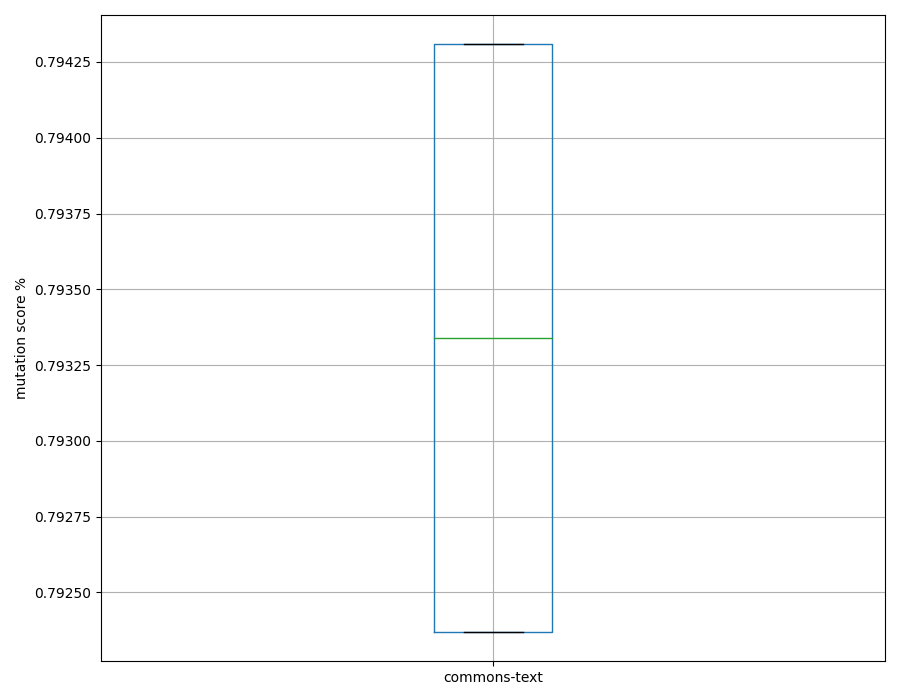
\includegraphics[scale=0.3]{images/full_75/boxplot_commons-text.png}}}
    \qquad
    \subfloat{{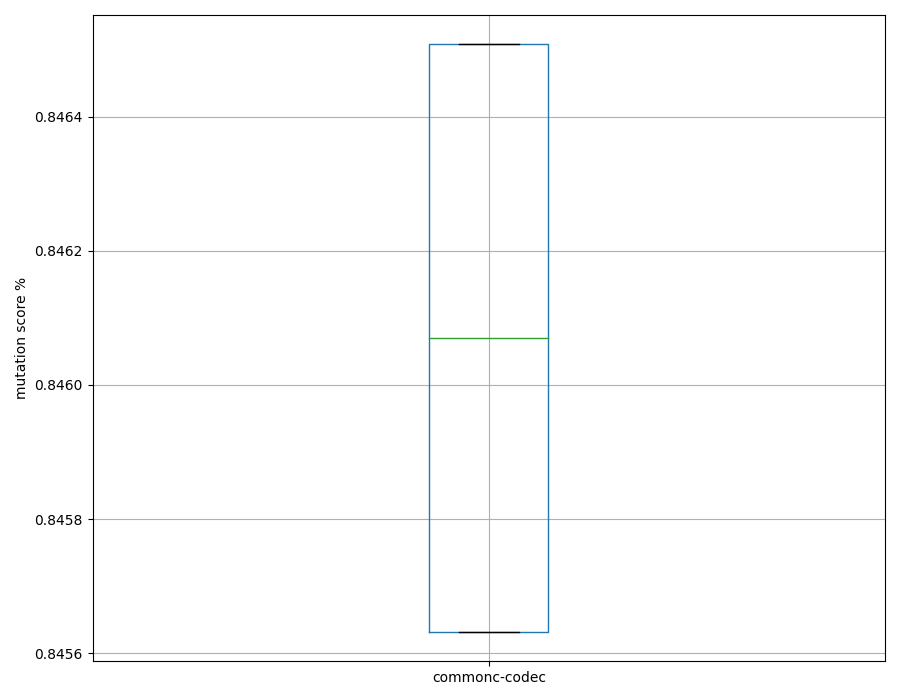
\includegraphics[scale=0.3]{images/full_75/boxplot_commonc-codec.png}}}
\end{figure}

\begin{figure}[h]
\centering
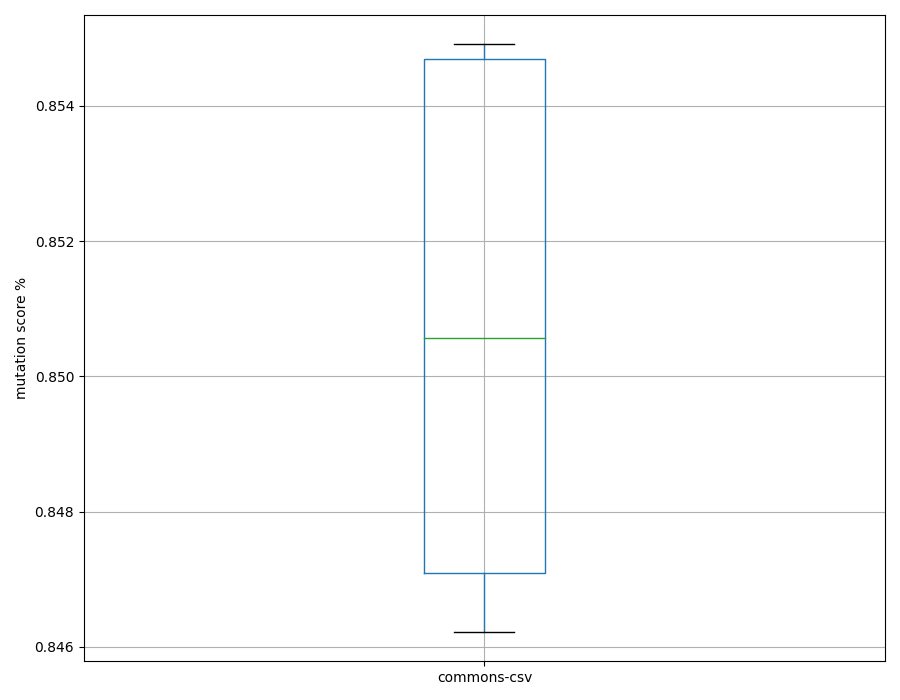
\includegraphics[scale=0.3]{images/full_75/boxplot_commons-csv.png}
\end{figure}


\chapter{Box-plots of samples per project without Levenshtein distance characteristic n*0.25 reduction}
\label{ap:no_distance_25}
\begin{figure}[h]
    \centering
    \subfloat{{\includegraphics[scale=0.32]{images/no_distance_25/boxplot_google-auto-service.png}}}
    \qquad
    \subfloat{{\includegraphics[scale=0.32]{images/no_distance_25/boxplot_scribejava-core.png}}}
\end{figure}

\begin{figure}[h]
    \centering
    \subfloat{{\includegraphics[scale=0.3]{images/no_distance_25/boxplot_google-auto-factory.png}}}
    \qquad
    \subfloat{{\includegraphics[scale=0.3]{images/no_distance_25/boxplot_google-auto-common.png}}}
\end{figure}

\begin{figure}[h]
    \centering
    \subfloat{{\includegraphics[scale=0.3]{images/no_distance_25/boxplot_google-auto-value.png}}}
    \qquad
    \subfloat{{\includegraphics[scale=0.3]{images/no_distance_25/boxplot_gson.png}}}
\end{figure}

\begin{figure}[h]
    \centering
    \subfloat{{\includegraphics[scale=0.3]{images/no_distance_25/boxplot_commons-io.png}}}
    \qquad
    \subfloat{{\includegraphics[scale=0.3]{images/no_distance_25/boxplot_commons-cli.png}}}
\end{figure}

\begin{figure}[h]
    \centering
    \subfloat{{\includegraphics[scale=0.3]{images/no_distance_25/boxplot_commons-text.png}}}
    \qquad
    \subfloat{{\includegraphics[scale=0.3]{images/no_distance_25/boxplot_commonc-codec.png}}}
\end{figure}

\begin{figure}[h]
\centering
\includegraphics[scale=0.3]{images/no_distance_25/boxplot_commons-csv.png}
\end{figure}

\chapter{Box-plots of samples per project without Levenshtein distance characteristic n*0.50 reduction}
\label{ap:no_distance_50}
\begin{figure}[h]
    \centering
    \subfloat{{\includegraphics[scale=0.32]{images/no_distance_50/boxplot_google-auto-service.png}}}
    \qquad
    \subfloat{{\includegraphics[scale=0.32]{images/no_distance_50/boxplot_scribejava-core.png}}}
\end{figure}

\begin{figure}[h]
    \centering
    \subfloat{{\includegraphics[scale=0.3]{images/no_distance_50/boxplot_google-auto-factory.png}}}
    \qquad
    \subfloat{{\includegraphics[scale=0.3]{images/no_distance_50/boxplot_google-auto-common.png}}}
\end{figure}

\begin{figure}[h]
    \centering
    \subfloat{{\includegraphics[scale=0.3]{images/no_distance_50/boxplot_google-auto-value.png}}}
    \qquad
    \subfloat{{\includegraphics[scale=0.3]{images/no_distance_50/boxplot_gson.png}}}
\end{figure}

\begin{figure}[h]
    \centering
    \subfloat{{\includegraphics[scale=0.3]{images/no_distance_50/boxplot_commons-io.png}}}
    \qquad
    \subfloat{{\includegraphics[scale=0.3]{images/no_distance_50/boxplot_commons-cli.png}}}
\end{figure}

\begin{figure}[h]
    \centering
    \subfloat{{\includegraphics[scale=0.3]{images/no_distance_50/boxplot_commons-text.png}}}
    \qquad
    \subfloat{{\includegraphics[scale=0.3]{images/no_distance_50/boxplot_commonc-codec.png}}}
\end{figure}

\begin{figure}[h]
\centering
\includegraphics[scale=0.3]{images/no_distance_50/boxplot_commons-csv.png}
\end{figure}

\chapter{Box-plots of samples per project without Levenshtein distance characteristic n*0.75 reduction}
\label{ap:no_distance_75}
\begin{figure}[h]
    \centering
    \subfloat{{\includegraphics[scale=0.32]{images/no_distance_75/boxplot_google-auto-service.png}}}
    \qquad
    \subfloat{{\includegraphics[scale=0.32]{images/no_distance_75/boxplot_scribejava-core.png}}}
\end{figure}

\begin{figure}[h]
    \centering
    \subfloat{{\includegraphics[scale=0.3]{images/no_distance_75/boxplot_google-auto-factory.png}}}
    \qquad
    \subfloat{{\includegraphics[scale=0.3]{images/no_distance_75/boxplot_google-auto-common.png}}}
\end{figure}

\begin{figure}[h]
    \centering
    \subfloat{{\includegraphics[scale=0.3]{images/no_distance_75/boxplot_google-auto-value.png}}}
    \qquad
    \subfloat{{\includegraphics[scale=0.3]{images/no_distance_75/boxplot_gson.png}}}
\end{figure}

\begin{figure}[h]
    \centering
    \subfloat{{\includegraphics[scale=0.3]{images/no_distance_75/boxplot_commons-io.png}}}
    \qquad
    \subfloat{{\includegraphics[scale=0.3]{images/no_distance_75/boxplot_commons-cli.png}}}
\end{figure}

\begin{figure}[h]
    \centering
    \subfloat{{\includegraphics[scale=0.3]{images/no_distance_75/boxplot_commons-text.png}}}
    \qquad
    \subfloat{{\includegraphics[scale=0.3]{images/no_distance_75/boxplot_commonc-codec.png}}}
\end{figure}

\begin{figure}[h]
\centering
\includegraphics[scale=0.3]{images/no_distance_75/boxplot_commons-csv.png}
\end{figure}







	
\end{appendices}